\documentclass[12pt]{report}

\usepackage[letterpaper, margin=1truein, footskip=.25in, twoside]{geometry}
\usepackage[utf8]{inputenc}
\usepackage[english]{babel}

\usepackage{setspace}
\doublespacing

% Header and footer
\usepackage{fancyhdr}
\pagestyle{fancy}
\fancyhead{}
\fancyhead[RO,LE]{\thepage}
\fancyhead[RE]{\it\leftmark}
\fancyhead[LO]{\it\rightmark}
\fancyfoot{}

% Figures and images
\usepackage{graphicx}
\graphicspath{ {images/} }
\usepackage{color}
\usepackage[font={small,it}]{caption}
\usepackage{epsfig}
\usepackage{epstopdf}

\usepackage{amsmath}
\usepackage{amsfonts}
\usepackage{amssymb}
\usepackage{url}
\usepackage{array}

\usepackage{amsthm}
\theoremstyle{plain}
\newtheorem{thm}{Theorem}[section]
\newtheorem{lem}[thm]{Lemma}
\newtheorem{prop}[thm]{Proposition}
\newtheorem*{cor}{Corollary}
\newtheorem{subclaim}{Claim}[subsubsection]

\theoremstyle{definition}
\newtheorem{defn}{Definition}[section]
\newtheorem{conj}{Conjecture}[section]
\newtheorem{exmp}{Example}[section]

\theoremstyle{remark}
\newtheorem*{rem}{Remark}
\newtheorem*{conv}{Convention}

\usepackage{tikz}
\usetikzlibrary{calc}

% Custom commands
\newcommand{\abs}[1]{\left|#1\right|}
\newcommand{\Conf}{\mathrm{Conf}}
\newcommand{\DConf}{\mathrm{Conf}^{\,\square}}
\newcommand{\UConf}{\mathrm{UConf}}

\begin{document}

% Title, Abstract, and Acknowledgements
\begin{titlepage}
   \begin{center}
       \vspace*{\fill}
       {GRAPH CONFIGURATION SPACES AND BRAID GROUPS}
 
       \vspace{1cm}
 
       A THESIS\\
       SUBMITTED TO THE GRADUATE SCHOOL\\
       IN PARTIAL FULFILLMENT OF THE REQUIREMENTS\\
       FOR THE DEGREE\\
       MASTER OF SCIENCE\\
       BY\\
       ZACH WILCHER\\
       DR. JUSTIN MURRAY - ADVISOR
 
       \vspace{1 cm}
 
       BALL STATE UNIVERSITY\\
       MUNCIE, INDIANA\\
       MAY 2026
       \vspace*{\fill}
   \end{center}
\end{titlepage}
\clearpage\shipout\null
\pagenumbering{roman}
\chapter*{Abstract}
{\bf THESIS:} Graph Configuration Spaces and Braid Groups
\\{\bf STUDENT:} Zach Wilcher
\\{\bf DEGREE:} Master of Science
\\{\bf COLLEGE:} Sciences and Humanities
\\{\bf DATE:} May 2026
\\{\bf PAGES:} \pageref{LastPage}
\\
Given any space \(X\), the \(n\) point configuration space \(\Conf_n(X)\) is 
\(X^n - \Delta\), where \(\Delta\) is the diagonal in \(X^n\). 
Contrast this with the \(n\) point unordered configuration space \(\UConf_n(X) = \Conf_n(X) / S_n\)
where the quotient is obtained by permuting the coordinates of points in \(\Conf_n(X)\).
The fundamental groups of \(\Conf_n(X)\) and \(\UConf_n(X)\) are respectively known as the \(n\)-strand pure braid group
\(P_n(X)\) and the \(n\)-strand braid group \(B_n(X)\).
The base point will be omitted since the considered spaces are path connected.

\(B_n(\mathbb{R}^2)\) is also known as the Artin braid group and has applications
in motion planning, fluid mechanics, and quantum information theory.
Ghirst and Koditschek showed in 1999 that using a graph \(\Gamma\) as the underlying space has 
been applied to modeling the paths of automated guided vehicles.

Topologically, \(\Conf_n(\Gamma)\) is an interesting space in its own right. 
Abrams showed in 2000 that \(\Conf_2(\Gamma)\) is a surface if and only if \(\Gamma\)
is the complete \(5\) graph \(K_5\), or the bipartite graph \(K_{3,3}\).
By constructing the neighborhoods of each vertex in the configuration space
and computing the Euler characteristic, it can be shown
whether the space is a surface and what kind of surface it is.
The goals for this project are to 
find new examples of surfaces arising from \(\Conf_n(\Gamma)\) when \(n > 2\),
and to determine precisely which graphs yield surfaces when \(n > 2\).
\chapter*{Acknowledgements}
\tableofcontents
\clearpage\shipout\null
\pagenumbering{arabic}

% Content Chapters
\chapter{Configuration Spaces}

\section{Definitions and preliminary results}
% These definitions are presented in Abrams on page 10.
Given a topological space \(X\), the \(n\) point (topological) configuration space of \(X\) is
\(\Conf_n(X) = X^n - \Delta\) where \(\Delta\) is the diagonal in \(X^n\).

Treating a graph \(\Gamma\) as a topological space we can construct the
\(n\) point discretized or combinatorial configuration space \(\DConf_n(\Gamma)\) by 
% this diagonal needs elaboration.
removing a larger diagonal \(\Delta^{\square} = \{(e_1, \ldots, e_n) \mid x_i \cap x_j \neq \emptyset \text{ for some } i \neq j\}\)
from \(\Gamma^n\). Here \((e_1, \cdots, e_n)\) is any \(n\)-tuple of cells in \(\Gamma\).

Abrams showed in \cite{abrams2000configurationspaces} that \(\Conf_n(\Gamma)\) deformation retracts onto \(\DConf_n(\Gamma)\) and
that \(\DConf_n(\Gamma)\) is a cubical complex.
He also notes that any point in the
\(n\)-point configuration space is in one-to-one correspondence with a
collection of ``tokens'' placed on the graph. In this project, we will use a slightly different terminology and
and say ``particles'' instead of ``tokens.''

% TODO what is a cubical complex?
% make sure to define n-cubes and the gluing map

\begin{figure}[h!]
\centering
\begin{tikzpicture}
    \node (u1) at (2, 2) {\(u_1\)};
    \node (u2) at (4, 2) {\(u_2\)};
    \node (u3) at (3, 1) {\(u_3\)};
    \node (u4) at (3, 0) {\(u_4\)};
    \draw (u1) -- (u3);
    \draw (u2) -- (u3);
    \draw (u4) -- (u3);
\end{tikzpicture}
\caption{The \(Y\)-graph}
\label{fig:ygraph}
\end{figure}
Imagine \(2\) particles placed on the graph in \ref{fig:ygraph} at \(u_1\) and \(u_2\).  
In the topological configuration space, as the particle at \(u_1\) moves to \(u_3\)
the particle at \(u_2\) is free to simultaneously move to \(u_3\) as well. 
However, both particles would not be able to occupy the vertex \(u_3\) simultaneously.  
Compare this with the combinatorial configuration space, as the
particle at \(u_1\) moves to \(u_3\), the particle at \(u_2\) can not move at
all since the edges \(u_1 u_3\) and \(u_2 u_3\) intersect at \(u_3\) and points
with coordinates belonging to both edges are removed.

\begin{figure}[h!]
\centering
\begin{tikzpicture}
    \node (v1) at (0, 2) {\(v_1\)};
    \node (v2) at (0, 0) {\(v_2\)};
    \draw (v1) -- (v2);
    \node (u1) at (2, 2) {\(u_1\)};
    \node (u2) at (4, 2) {\(u_2\)};
    \node (u3) at (3, 1) {\(u_3\)};
    \node (u4) at (3, 0) {\(u_4\)};
    \draw (u1) -- (u3);
    \draw (u2) -- (u3);
    \draw (u4) -- (u3);
\end{tikzpicture}
\caption{An edge and a \(Y\)-graph}
\label{fig:edgeygraph}
\end{figure}
Now consider the graph in figure \ref{fig:edgeygraph} and put particles at \(v_1\) and \(u_3\).
As the particle at \(v_1\) moves to \(v_2\) there are three ways that the particle at \(u_3\) can move.
Since each way that the particle at \(u_3\) can move can be done simultaneously as the movement of the particle at \(v_1\),
the \(1\)-cell corresponding to the movement of the particle at \(v_1\) to \(v_2\)
borders three distinct \(2\)-cubes (see figure \ref{fig:threepagebook}).
We call this structure a \(3\)-page book.

\begin{figure}[h!]
\centering
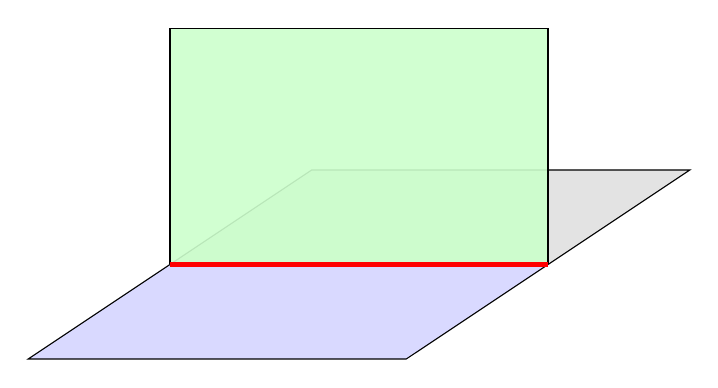
\begin{tikzpicture}[
    scale=1.2,
    % Define a 3D-like perspective by setting the coordinate vectors.
    % x goes to the right, y goes up, and z gives a sense of depth.
    z={(-0.6cm,-0.4cm)}, 
    x={(1cm,0cm)},      
    y={(0cm,1cm)}       
]
    % --- Define Coordinates for the vertices of the book ---
    
    % The spine is a 1-cell from O to A
    \coordinate (O) at (0,0,0);
    \coordinate (A) at (4,0,0);

    \coordinate (B_Back) at (4,0,-2.5);
    \coordinate (C_Back) at (0,0,-2.5);

    \coordinate (B_Front) at (4,0,2.5);
    \coordinate (C_Front) at (0,0,2.5);

    \coordinate (B_Up) at (4,2.5,0);
    \coordinate (C_Up) at (0,2.5,0);

    % Draw book pages
    \fill[gray!30, opacity=0.75] (O) -- (A) -- (B_Back) -- (C_Back) -- cycle;
    \draw (O) -- (C_Back) -- (B_Back) -- (A);

    \fill[blue!20, opacity=0.75] (O) -- (A) -- (B_Front) -- (C_Front) -- cycle;
    \draw (O) -- (C_Front) -- (B_Front) -- (A);

    \fill[green!20, opacity=0.9] (O) -- (A) -- (B_Up) -- (C_Up) -- cycle;
    \draw (O) -- (C_Up) -- (B_Up) -- (A);

    % --- Draw the Spine on top so it stands out ---
    \draw[line width=1.5pt, red] (O) -- (A);
\end{tikzpicture}
\caption{A 3-page book}
\label{fig:threepagebook}
\end{figure}

% It would make so much more sense if we excluded the covers of the book when counting the pages.
% Then, a book with more than 0 pages is not homeomorphic to a surface. 
% However, this would be an annoying substitution in later proofs.
\begin{defn}
    An \(n\)-page book is a collection of \(n\) \(2\)-cubes each glued along a common edge.
    This edge is called the spine of the book.
\end{defn}

Books are common structures found in configuration spaces.
One goal for this project is to determine which configuration spaces are surfaces.

\begin{thm}
A book with more than \(2\) pages is not a surface.
\end{thm}
\begin{proof}
Suppose there exists an \(n\)-page book that is a surface but \(n > 2\).
Let \(p\) be some point in the interior of the book's spine.
% pg. 225 Munkres states that an m-manifold X is a Hausdorff space such that for each point x in 
% X there exists a nehiborhood of x that is homeomorphic to an open subset of R^m.
% Let U be the neihborhood of p in X, V be the open subset of R^2, and \phi
% be the homeomorphism from U to V.
% Take some open disk B centered at \phi(p) in V such that \closure{B} \subseteq V
% restrict \phi to this open disk (this is okay to do in the codomain as \phi is a bijection).
Since the book is homeomorphic to a surface, there exists an open neighborhood \(U\) of \(p\)
which is homeomorphic to an open disk \(B\) in \(\mathbb{R}^2\).
Let \(\phi\) be a homeomorphism from \(\closure{U}\) to \(\closure{B}\) and \(S\) be the portion of book's spine inside of \(U\).
Notice that \(U \setminus S\) consists of \(n\) path components--one from each page of the book.
However,
\[
U\setminus S \cong \phi(U\setminus S) = B \setminus \phi(S).
\]

We claim that \(\phi(S)\) must separate \(B\) into two components.
To see this, first note that \(\phi(S)\) is a properly imbedded arc in \(B\) with \(\Bd(\phi(S))\) consisting of two
points on \(\Bd(B)\).
% homemorphisms map boundary points to boundary points, interior points to interior points, and exterior points to exterior points.
% This is common knowledge but a proof might be necessary TODO.
Since \(\Bd(B)\) is homeomorphic to a circle, there exists two different paths \(\alpha\) and \(\beta\) 
connecting these two points together (See Figure \ref{fig:thm:book_1_1}).

\begin{figure}[h!]
    \centering
    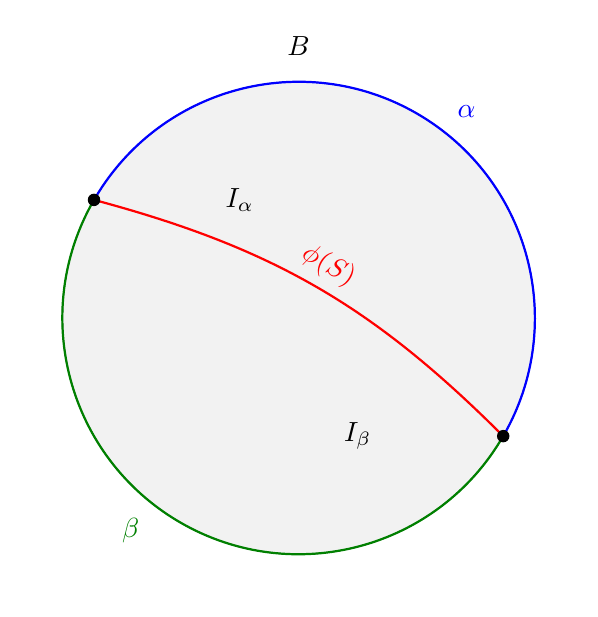
\begin{tikzpicture}[scale=1.5]
        % Define the main circle (the disk D^2) and fill it lightly
        \fill[gray!10] (0,0) circle (2cm);
        \draw (0,0) circle (2cm);
        \node at (0, 2.3) {\(B\)};

        % Define the start and end points of the arc on the boundary of the disk
        \coordinate (P1) at (150:2cm);
        \coordinate (P2) at (-30:2cm);

        % Draw the separating arc phi(S \cap U) with a distinct color
        \draw[thick, red] (P1) to[bend left=15] node[above, pos=0.5, sloped] {\(\phi(S)\)} (P2);

        % Draw the boundary path alpha
        \draw[thick, blue] (P2) arc (-30:150:2cm);
        \node[blue, above, xshift=18pt, yshift=-5pt] at (60:2cm) {\(\alpha\)};
        
        % Draw the boundary path beta
        \draw[thick, green!50!black] (P1) arc (150:330:2cm);
        \node[green!50!black, below, xshift=-18pt, yshift=5pt] at (240:2cm) {\(\beta\)};
        
        % Label the two regions separated by the arc
        \node at (-0.5, 1) {\(I_{\alpha}\)};
        \node at (0.5, -1) {\(I_{\beta}\)};
        
        % Mark the endpoints on the boundary
        \fill (P1) circle (1.5pt);
        \fill (P2) circle (1.5pt);

    \end{tikzpicture}
    \caption{The arc \(\phi(S)\) separates the open disk \(B\) into two components, \(I_{\alpha}\) and \(I_{\beta}\).}
    \label{fig:thm:book_1_1}
\end{figure}

The Jordan curve theorem guarantees that the simple closed curve \(\alpha \cup \phi(S)\) (resp. \(\beta \cup \phi(S)\))
separate \(B \setminus (\alpha \cup \phi(S))\) (resp. \(B \setminus (\beta \cup \phi(S))\)) into a bounded connected component
\(I_{\alpha}\) and an unbounded connected component \(O_{\alpha}\) (resp. \(I_{\beta}\) and \(O_{\beta}\)) when imbedded in \(\mathbb{R}^2\).
Notice \(B\setminus \phi(S) = I_{\alpha} \cup I_{\beta}\).
Since \(I_{\alpha} \subseteq O_{\beta}\) and \(I_{\beta} \cap O_{\beta} = \emptyset\),
we have that \(I_{\alpha} \cap I_{\beta} = \emptyset\).
So, \(I_{\alpha}\) and \(I_{\beta}\) form a separation of \(B\setminus \phi(S)\).
\end{proof}

Another common structure found found in graph configuration spaces are \(n\)-cubes.
Consider the graph in Figure \ref{fig:3edges} and imagine \(3\) particles placed at \(u_1\), \(v_1\), and \(w_1\).
Each particle can simultaneously move to \(u_2\), \(v_2\), and \(w_2\) resulting in \(3\)-cube in the configuration space (see Figure \ref{fig:3cube}).

\begin{figure}[h!]
    \centering
\begin{tikzpicture}
    \node (u1) at (0, 2) {\(u_1\)};
    \node (u2) at (0, 0) {\(u_2\)};
    \draw (u1) -- (u2);
    \node (v1) at (2, 2) {\(v_1\)};
    \node (v2) at (2, 0) {\(v_2\)};
    \draw (v1) -- (v2);
    \node (w1) at (4, 2) {\(w_1\)};
    \node (w2) at (4, 0) {\(w_2\)};
    \draw (w1) -- (w2);
\end{tikzpicture}
    \caption{Three edges}
    \label{fig:3edges}
\end{figure}

\begin{figure}[h!]
    \centering
    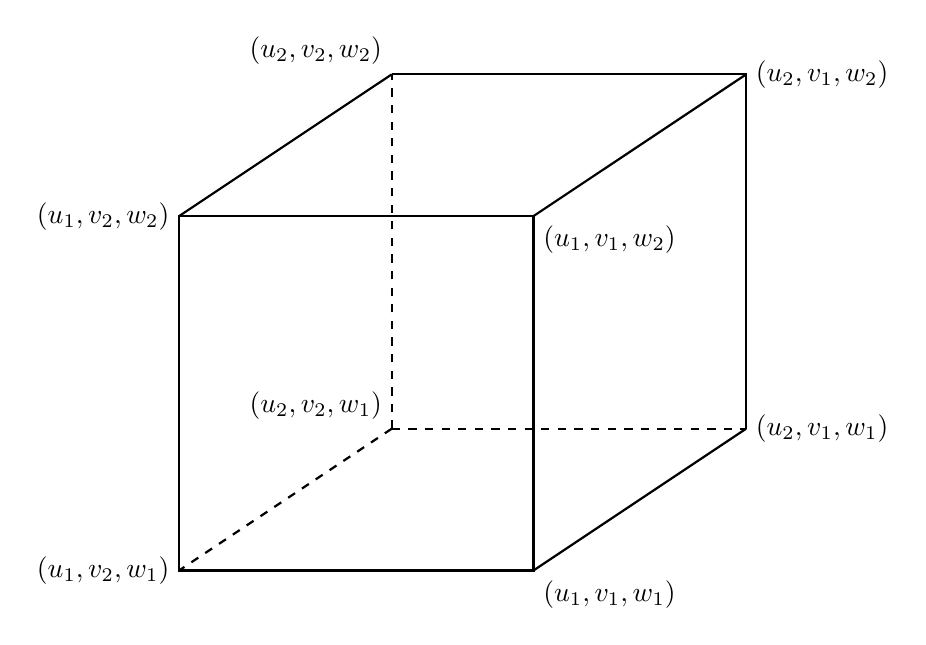
\begin{tikzpicture}[
    scale=1.5,
    % Define a 3D-like perspective by setting the coordinate vectors.
    % x goes to the right, y goes up, and z gives a sense of depth.
    x={(1cm,0cm)},
    y={(0cm,1cm)},
    z={(-0.6cm,-0.4cm)}
]
    % --- Style Definitions ---
    % Define styles for the cube's edges to make the code cleaner.
    % 'visible' edges are solid and thick.
    % 'hidden' edges are dashed and thick.
    \tikzstyle{visible} = [draw, thick, black]
    \tikzstyle{hidden} = [draw, thick, dashed, black]

    % --- Vertex Coordinates ---
    % Define the 8 vertices of the cube using (x,y,z) coordinates.
    % The side length of the cube is 3 units.
    \def\s{3}
    \coordinate (A) at (0,0,0);
    \coordinate (B) at (\s,0,0);
    \coordinate (C) at (\s,\s,0);
    \coordinate (D) at (0,\s,0);
    \coordinate (E) at (0,0,\s);
    \coordinate (F) at (\s,0,\s);
    \coordinate (G) at (\s,\s,\s);
    \coordinate (H) at (0,\s,\s);

    % --- Draw Hidden Edges ---
    % Draw the edges that would be obscured from view first. These are the
    % edges connected to the rearmost vertex (A).
    \draw[hidden] (A) -- (B);
    \draw[hidden] (A) -- (D);
    \draw[hidden] (A) -- (E);

    % --- Draw Visible Edges ---
    % Draw the visible edges on top of the hidden ones.
    \draw[visible] (B) -- (C) -- (D);
    \draw[visible] (E) -- (F) -- (G) -- (H) -- cycle;
    \draw[visible] (B) -- (F);
    \draw[visible] (C) -- (G);
    \draw[visible] (D) -- (H);

    % --- Optional: Label Vertices ---
    % Uncomment the following lines to add labels to each vertex.
    \node at (A) [above left] {\((u_2, v_2, w_1)\)};
    \node at (B) [right] {\((u_2, v_1, w_1)\)};
    \node at (C) [right] {\((u_2, v_1, w_2)\)};
    \node at (D) [above left] {\((u_2, v_2, w_2)\)};
    \node at (E) [left] {\((u_1, v_2, w_1)\)};
    \node at (F) [below right] {\((u_1, v_1, w_1)\)};
    \node at (G) [below right] {\((u_1, v_1, w_2)\)};
    \node at (H) [left] {\((u_1, v_2, w_2)\)};    
\end{tikzpicture}
\caption{3-cube}
\label{fig:3cube}
\end{figure}

Visually \(n\)-cubes are ``clearly'' not surfaces when \(n > 2\).
However, we can show this formally with an argument using the fundamental group.
\begin{thm}
\(n\)-cubes are not surfaces when \(n > 2\).
\end{thm}
\begin{proof}
    Suppose an \(n\)-cube \(C\) is a surface for some \(n > 2\).
    % imbed C in R^n
    Pick some point \(p\) in the interior of \(C\).
    Since \(C\) is a surface there exists some open ball \(B^n(p, \epsilon)\) in the interior of \(C\) such that 
    it is centered at \(p\) and is homeomorphic to some open neighborhood \(V\) of \(\mathbb{R}^2\).
    Let \(q\) be the point in \(V\) corresponding to \(p\).
    
    % TODO just use the fact that local simple connectedness fails after removing a point in D^2 but doesn't after removing a point in S^2.
\end{proof}

Books and cubes are the meat and potatos of the coming proofs.

\section{Computing the Euler characteristic of graph configuration spaces}
To compute the euler characteristic of an unorderd \(n\) point graph configuration space we need to count
for each \(0 \le k \le n\) the number of \(k\)-cubes present.
Without further mention \(E = E(\Gamma)\) and \(V = V(\Gamma)\).

A \(k\) cube exists if and only if \(k\) particles are free to move simultaneously while \(n - k\)
particles remain fixed.
Hence the general formula for the number of \(k\) cubes in \(\DUConf_n(\Gamma)\) is
\[
    \abs{\phi(k)} \cdot \begin{pmatrix}\abs{V} - 2k \\ n - k\end{pmatrix}
\]
where \(\phi(k)\) defined as follows.

\begin{defn}
\(\phi(k)\) is the collection consisting of all unordered sets of exactly \(k\) disjoint edges in \(\Gamma\)
where \(\phi(0) = \{\emptyset\}\).
\end{defn}

Note that we define \(\phi(0) = \{\emptyset\}\) so that \(\abs{\phi(0)} = 1\).
With this definition, \(\abs{\phi(k)}\) is also known as the number of ``\(k\)-matchings'' in \(\Gamma\).

Counting the number of \(k\)-matchings for small graphs can be done efficiently 
with a simple sweep over all \(k\) combinations of edges.
However, for general larger graphs this computation quickly becomes unwieldly.

% TODO read/cite Mark Jerrum's paper "Two-dimensional monomer-dimer systems are computationally intractable"
% where he proves computing the matching polynomial for planar graphs is P# ?
% TODO: reference program actually used to make computations? It's trivial especially now with AI hah

\begin{figure}[h!]
\centering
\begin{tabular}{c | c | c}
   \(\Gamma\) & \(n\) & \(\chi(\DUConf_n(\Gamma))\) \\
   \hline
   \(K_5\) & 2 & -5 \\
   \(K_{3,3}\) & 2 & -3 \\
   \(K_5\) & 3 & -5 \\
   \(\Theta_4\) & 3 & -4 \\
   \(K_{3,3}\) & 4 & -3
\end{tabular}
\label{fig:euler_characteristics}
\caption{Euler characteristic of certain unordered graph configuration spaces.}
\end{figure}

A workaround for this computational challenge is determing the Euler characteristic of certain classes of graphs.
In \cite{appiah2024algebraicstructurehyperbolicgraph} the ``pulsar'' graph was defined.


\begin{figure}[h!]
    \centering
\begin{tikzpicture}[scale=1]
    % Define the two main suspension vertices, positioned closer together
    \node (a1) at (0, 1) {\(a_1\)};
    \node (a2) at (0, -1) {\(a_2\)};

    % Define the intermediate vertices for the 'm' paths
    \node (b1) at (-1, 0) {\(b_1\)};
    \node (bm) at (1, 0) {\(b_m\)};
    \node at (0,0) {\(\dots\)};

    % Draw the edges for the 'm' paths, passing through the b_i nodes
    \draw (a1) to[out=180, in=90] (b1);
    \draw (b1) to[out=270, in=180] (a2);

    \draw (a1) to[out=0, in=90] (bm);
    \draw (bm) to[out=270, in=0] (a2);

    % Define vertices for the 'n1' rays attached to a1, spread out as in the drawing
    \node (c1) at (-1, 2) {\(c_1\)};
    \node (c1p) at (-2, 3) {\(c'_1\)};
    \node (cn1) at (1, 2) {\(c_{n_1}\)};
    \node (cn1p) at (2, 3) {\(c'_{n_1}\)};
    \node at (0, 2.5) {\(\dots\)};

    % Draw edges for the 'n1' rays
    \draw (a1) -- (c1);
    \draw (c1) -- (c1p);
    \draw (a1) -- (cn1);
    \draw (cn1) -- (cn1p);

    % Define vertices for the 'n2' rays attached to a2, also spread out
    \node (d1) at (-1, -2) {\(d_1\)};
    \node (d1p) at (-2, -3) {\(d'_1\)};
    \node (dn2) at (1, -2) {\(d_{n_2}\)};
    \node (dn2p) at (2, -3) {\(d'_{n_2}\)};
    \node at (0, -2.5) {\(\dots\)};

    % Draw edges for the 'n2' rays
    \draw (a2) -- (d1);
    \draw (d1) -- (d1p);
    \draw (a2) -- (dn2);
    \draw (dn2) -- (dn2p);
\end{tikzpicture}
\label{fig:pulsargraph}
\caption{The Pulsar graph \(\mathcal{P}_{m,n_1,n_2}\)}
\end{figure}

\begin{thm}
    \label{thm:pulsargrapheuler}
    The Euler characteristic of \(\DUConf_{3}(\mathcal{P}_{m,n_1,n_2})\) is
    \[
    \frac{m^{3}}{6} - \frac{3 m^{2}}{2} - \frac{m n_{1}^{2}}{2} - \frac{3 m n_{1}}{2} - \frac{m n_{2}^{2}}{2} - \frac{3 m n_{2}}{2} + \frac{7 m}{3} - \frac{n_{1}^{3}}{3} + \frac{7 n_{1}}{3} - \frac{n_{2}^{3}}{3} + \frac{7 n_{2}}{3}.
    \]
\end{thm}
\begin{proof}
%TODO: all we really have to do is explain the argument for the 2 and 3 matchings.
\end{proof}

\begin{rem}
Substituting in \(n_1 = 0\) and \(n_2 = 0\) the pular graph becomes \(\Theta_m\).
So, 
the euler characteristic of \(\DUConf_3(\Theta_m)\) is
\[
\frac{m^{3}}{6} - \frac{3 m^{2}}{2} + \frac{7 m}{3}
\]
This aligns with results in section 4 of \cite{appiah2024algebraicstructurehyperbolicgraph}.
\end{rem}
\chapter{Surfaces}
In his thesis \cite{abrams2000configurationspaces}, Abrams asked:
For which \(n\) and \(\Gamma\) is \(\DConf_n(\Gamma)\) homeomorphic to a closed manifold?
He establishes a partial answer to this question in Corollary 5.8: 
if \(\Gamma\) is a connected graph
without loops and \(\DConf_n(\Gamma)\) is homeomorphic to a closed
\(n\)-dimensional manifold, then either \(n = 1\) and \(\Gamma\) is a cycle, or
\(n = 2\) and \(\Gamma\) is \(K_5\) or \(K_{3,3}\).

Advised by Peter Haskell, Praphat Fernandes in his undergraduate thesis
demonstrates that if \(\Gamma\) is a simple graph and \(\DConf_2(\Gamma)\)
is a \(2\)-psuedomanifold without boundary the following are true.
\begin{enumerate}
    \item If \(\Gamma\) contains a valence 4 vertex, then \(\Gamma\) is \(K_5\).
    \item If every vertex in \(\Gamma\) has valence 3, then \(\Gamma\) is \(K_{3,3}\).
\end{enumerate}
This recovers Abrams' result about when \(\DConf_2(\Gamma)\) 
is a \(2\)-manifold, as Praphat also shows that
if \(\Gamma\) is simple and \(\DConf_2(\Gamma)\) is a 2-psuedomanifold without boundary,
then the valence of every vertex in \(\Gamma\) is between 3 and 4,
and \(\DConf_2(\Gamma)\) is a 2-manifold. Also advised by Peter Haskell, Molly Ison in \cite{ison2005two} 
extends Fernandes' work in her masters thesis to 2-psuedomanifolds with boundary.

% TODO: is it though?
The question for when \(\DConf_n(\Gamma)\) is an \(m\)-manifold 
when \(n \neq m\) remains open.

In Example 4.3 in \cite{ko2012characteristics}, it is shown that \(\DConf_3(\Theta_4)\)
is a closed orientable surface of genus 3 by computing its fundamental group and using the
fact that discretized configuration spaces are \(K(\pi, 1)\) spaces.
This result is recovered in \cite{appiah2024algebraicstructurehyperbolicgraph}
with a strictly combinatorial argument.

The goal of this chapter is to
answer for what \(\Gamma\) and what \(n\) is
\(\DConf_n(\Gamma)\) is a \(2\)-manifold without boundary.

\section{Proofs of surfacedom}

% TODO prove explicitly that these graphs are surfaces.

\section{Ruling out other graphs}
The example graphs in the previous section are in fact the only connected graphs
whose discretized configuration spaces are surfaces.

\begin{lem}
\label{lem:is_surface_0}
If \(\DConf_n(\Gamma)\) is an \(m\)-manifold with or without boundary, then \(\Gamma\) has at least \(n+m\) vertices.
\end{lem}
\begin{proof}
    If \(\Gamma\) has less than \(n\) vertices, then \(\DConf_n(\Gamma)\) is empty;
    so, suppose \(\Gamma\) has at least \(n\) vertices.
    If \(\Gamma\) has less than \(n + m\) vertices, then
    for any configuration of \(n\) particles on \(\Gamma\)
    at most \(m-1\) particles can simultaneously move.
    Since exactly \(m\) particles need to be able to simultaneously move for an \(m\)-cube 
    to exist in \(\DConf_n(\Gamma)\), no configuration in \(\DConf_n(\Gamma)\)
    can have a neighborhood homeomorphic to an open set in \(\mathbb{R}^m\).
\end{proof}

\begin{lem}
    \label{lem:is_connected_0}
    If \(\DConf_n(\Gamma)\) is connected, then \(\Gamma\) has at least \(n + 1\) vertices
    and \(\Gamma\) is connected.
\end{lem}
\begin{proof}
    Suppose \(\DConf_n(\Gamma)\) is connected.
    If \(\Gamma\) has less than \(n + 1\) vertices, then \(\DConf_n(\Gamma)\) is either empty or
    consists of \(n!\) isolated points; so, \(\Gamma\) must have at least \(n+1\) vertices.

    Let \(v_1\) and \(v_2\) be distinct vertices in \(\Gamma\).
    To construct a path in \(\Gamma\) between \(v_1\) and \(v_2\), first let \(w_1, \ldots, w_{n-1}\)
    be \(n-1\) vertices in \(\Gamma\) distinct from \(v_1\) and \(v_2\).
    Next, since \(\DConf_n(\Gamma)\) is connected, there must be a path \(\gamma\)
    in \(\DConf_n(\Gamma)\) between the configurations
    \((v_1, w_1, \ldots, w_{n-1})\) and \((v_2, w_1, \ldots, w_{n-1})\).
    The path \(\gamma\) corresponds to a sequence of (potentially simultaneous) movements of particles on \(\Gamma\).
    In particular the particle at \(v_1\) must be able to eventually move to \(v_2\).
    The sequence of edges traveled by this particle gives a path in \(\Gamma\) between \(v_1\) and \(v_2\).
\end{proof}


\begin{lem}
    \label{lem:is_surface_1}
    Suppose \(\DConf_n(\Gamma)\) is a \(2\)-manifold without boundary and let
    \(v_1\) and \(w_1\) be adjacent vertices in \(\Gamma\). For any collection
    of \(n-1\) vertices \(\{v_2, \cdots, v_n\}\) in \(\Gamma - \{v_1, w_1\}\)
    there exists exactly two edges \(e_1 = v_i w_2\) and \(e_2 = v_j w_3\) such that
    \begin{enumerate}[label=(\roman*)]
        \item \(v_i\) and \(v_j\) belong to \(\{v_2, \cdots, v_n\}\)
        \item \(w_2\) and \(w_3\) fall outside of \(\{w_1, v_1, \cdots, v_n\}\)
        \item exactly one of the following hold in Figure \ref{fig:lem:is_surface_1_1}.
    \end{enumerate}

\begin{figure}[h!]
    \centering
        \begin{enumerate*}[label=(\arabic*)]
            \item \label{fig:lem:is_surface_1_1:1}
            \begin{minipage}{.3\textwidth}
                \centering
                \(v_i = v_j\) \textit{and} \(w_2 \neq w_3\) \\
                \vspace{1em}
                \begin{tikzpicture}
                \node (v1) at (0,2) {\(v_1\)};
                \node (w1) at (0,0) {\(w_1\)};
                \draw (v1) -- (w1);
                \node (vi) at (3, 2) {\(v_i\)};
                \node (w2) at (2, 0) {\(w_2\)};
                \node (w3) at (4, 0) {\(w_3\)};
                \draw (vi) -- (w2) node[midway, left] {\(e_1\)};
                \draw (vi) -- (w3) node[midway, right] {\(e_2\)};
                \end{tikzpicture} 
            \end{minipage}
            \hspace{3em}

            \item \label{fig:lem:is_surface_1_1:2}
            \begin{minipage}{.3\textwidth}
                \centering
                \(w_2 = w_3\) \textit{and} \(v_i \neq v_j\) \\
                \vspace{1em}
                \begin{tikzpicture}
                    \node (v1) at (0,2) {\(v_1\)};
                    \node (w1) at (0,0) {\(w_1\)};
                    \draw (v1) -- (w1);
                    \node (vi) at (2, 2) {\(v_i\)};
                    \node (vj) at (4, 2) {\(v_j\)};
                    \node (w2) at (3, 0) {\(w_2\)};

                    \draw (vi) -- (w2) node[midway, left] {\(e_1\)};
                    \draw (vj) -- (w2) node[midway, right] {\(e_2\)};
                \end{tikzpicture}
            \end{minipage}
        \end{enumerate*}
    \caption{Lemma \ref{lem:is_surface_1} possibilities.}
    \label{fig:lem:is_surface_1_1}
\end{figure}
\end{lem}
\begin{proof}
    Let \(v_2, \cdots, v_n\) be \(n-1\) vertices in \(\Gamma - \{v_1, w_1\}\).   
    Now, put a particle at each of the vertices \(v_1, \cdots, v_n\).
    Since no particle exists at \(w_1\) and \(v_1\) is adjacent to \(w_1\), 
    the particle at \(v_1\) can travel from \(v_1\) to \(w_1\).
    This particles movement corresponds to a \(1\)-cube in \(\DConf_n(\Gamma)\).
    Since the configuration space is a \(2\)-manifold without boundary, 
    this \(1\)-cube must border exactly two distinct \(2\)-cubes.
    For this \(1\)-cube to border some \(2\)-cube,
    there must be another particle at some vertex \(v_i \in \{v_2, \ldots, v_n\}\) that can move to some vertex
    \(w_2 \not \in \{w_1, v_1, \ldots, v_n\}\).
    Furthermore, since this \(1\)-cube needs to border two \(2\)-cubes, 
    the movement of the particle from \(v_i\) to \(w_2\) cannot be the only other movement in addition to
    the movement of the particle from \(v_1\) to \(w_1\). 
    Let \(v_j\) and \(w_3\) be the vertices corresponding to this other movement.
    
    Notice that if \(v_i \neq v_j\) and \(w_2 \neq w_3\), then as the particle at \(v_1\) travels to \(w_1\), the particles
    at \(v_i\) and \(v_j\) can simultaneously travel to \(w_2\) and \(w_3\) respectively. These three simultaneous movements correspond
    to a \(3\)-cube in \(\DConf_n(\Gamma)\) with the point \((v_1, \cdots, v_n)\) as a corner.
    Since \(\DConf_n(\Gamma)\) is assumed to be a \(2\)-manifold and \(e_1\) and \(e_2\) are distinct, 
    the result follows.
\end{proof}

The idea that every \(1\)-cube in our cubical complex must border exactly two distinct \(2\)-cubes
for it to be homeomorphic to a \(2\)-manifold without boundary can be generalized to
\(m\)-manifolds without boundary. In the next section we explore this idea further.
% TODO DELETE THIS IF WE DON'T ACTUALLY EXPLORE IT FURTHER!!!!!!!!!!!!!!
% Also, put a link to this section if we do.

\begin{lem}
    \label{lem:is_surface_2}
    Suppose \(\DConf_n(\Gamma)\) is a \(2\)-manifold without boundary for some \(n \ge 3\) and let \(v_1\) and \(w_1\) be adjacent vertices in \(\Gamma\).
    Let \(\{v_2, \cdots, v_n\}\) be a collection of \(n-1\) vertices in \(\Gamma - \{v_1, w_1\}\) 
    and \(e_1 = v_i w_2\), \(e_2 = v_j w_3\) be the edges guaranteed
    from applying Lemma \ref{lem:is_surface_1} to \(\{v_2, \cdots, v_n\}\) in \(\Gamma - \{v_1, w_1\}\).
    Then, exactly one of the following is true.
    \begin{enumerate}
        \item \(n = 3\) and these edges belong to a \(Y\)-graph in \(\Gamma - \{v_1, w_1\}\) with two vertices not in \(\{v_2, \cdots, v_n\}\).
        \item \(e_1\) and \(e_2\) belong to a \(3\)-cycle in \(\Gamma - \{v_1, w_1\}\) with two vertices not in \(\{v_2, \cdots, v_n\}\).
        \item \(e_1\) and \(e_2\) belong to an \(m\)-cycle in \(\Gamma - \{v_1, w_1\}\) with one vertex not in \(\{v_2, \cdots, v_n\}\) and \(4 \le m \le n\).
    \end{enumerate}
\end{lem}
\begin{proof}
    The argument proceeds by cases on the possibilities for the edges \(e_1\) and \(e_2\).
    
    \textbf{Case 1:} \(v_i = v_j\) (See \ref{fig:lem:is_surface_1_1:1} in Figure \ref{fig:lem:is_surface_1_1}). 
    In this case, \(e_1 = v_i w_2\) and \(e_2 = v_i w_3\). 
    Let \(v_k\) be some vertex in \(\{v_2, \cdots, v_n\}\setminus\{v_i\}\).
    Applying Lemma \ref{lem:is_surface_1} to \(\{w_2, v_2, \cdots, v_n\}\setminus\{v_k\}\) in \(\Gamma - \{v_1, w_1\}\),
    we obtain two new edges \(e_3\) and \(e_4\).
    Since \(e_2\) already connects \(v_i\) to \(w_3\) and there must be exactly two edges
    with exactly one endpoint in \(\{w_2, v_2, \cdots, v_n\}\setminus\{v_k\}\),
    one of \(e_3\) or \(e_4\) is \(e_2\). 
    Without a loss of generality suppose \(e_4 = e_2\).
    Since \(e_3\) must share an endpoint with \(e_4 = e_2\), it follows that \(e_3\) has either \(v_i\) as an endpoint or \(w_3\) as an endpoint (See Figure \ref{fig:lem:is_surface_2_0}).
    \begin{figure}[h!]
        \centering
        \begin{tikzpicture}
            \node (v1) at (0,2) {\(v_1\)};
            \node (w1) at (0,0) {\(w_1\)};
            \draw (v1) -- (w1);
            \node (vi) at (3, 2) {\(v_i\)};
            \node (w2) at (2, 0) {\(w_2\)};
            \node (w3) at (4, 0) {\(w_3\)};
            \draw (vi) -- (w2) node[midway, left] {\(e_1\)};
            \draw (vi) -- (w3) node[midway, right] {\(e_2\)};
            
            \node (vk) at (5, 2) {\(?\)};
            \draw (vi) -- (vk) node[midway, above] {\(e_3\)};
        \end{tikzpicture}
        \quad\quad
        \begin{tikzpicture}
            \node (v1) at (0,2) {\(v_1\)};
            \node (w1) at (0,0) {\(w_1\)};
            \draw (v1) -- (w1);
            \node (vi) at (3, 2) {\(v_i\)};
            \node (w2) at (2, 0) {\(w_2\)};
            \node (w3) at (4, 0) {\(w_3\)};
            \node (q) at (6, 0) {\(?\)};
            \draw (vi) -- (w2) node[midway, left] {\(e_1\)};
            \draw (vi) -- (w3) node[midway, right] {\(e_2\)};
            \draw (q) -- (w3) node[midway, below] {\(e_3\)};
            
        \end{tikzpicture}
        \caption{Possibilities if \(v_i = v_j\)}
        \label{fig:lem:is_surface_2_0}
    \end{figure}

    Lemma \ref{lem:is_surface_1} guarantees two facts about the edges we have so far.
    \begin{enumerate}
        \item \(e_1\) and \(e_2\) are the only edges with exactly one endpoint in \(\{v_2, \cdots, v_n\}\).
        \item \(e_3\) and \(e_4 = e_2\) are the only edges with exactly one endpoint in \(\{w_2, v_2, \cdots, v_n\}\setminus\{v_k\}\).
    \end{enumerate}
    We claim that if \(e_3\) has \(v_i\) as an endpoint, then \(v_k\) must be the other endpoint of \(e_3\)
    (see the graph on the left in Figure \ref{fig:lem:is_surface_2_1}).
    To verify this claim, suppose \(e_3\) has \(v_i\) as an endpoint and let \(v^*\) be the other endpoint of \(e_3\).
    Since \(e_3 \neq e_1\) and \(e_3 \neq e_2\) but \(e_3\) has \(v_i\) as an endpoint, the first fact above 
    guarantees that \(v^* \in \{v_2, \cdots, v_n\}\).
    The second fact guarantees that \(v^* \not \in \{w_2, v_2, \cdots, v_n\}\setminus\{v_k\}\).
    Hence,
    \[
        v^* \in \left(V(\Gamma - \{v_1, w_1\})\setminus(\{w_2, v_2, \cdots, v_n\}\setminus\{v_k\})\right) \cap \{v_2, \cdots, v_n\} = \{v_k\}.
    \]

    Moreover, if \(e_3\) has \(v_i\) as an endpoint, 
    then since \(v_k\) was arbitrary, 
    every vertex in \(\{v_2, \cdots, v_n\}\setminus\{v_i\}\) is adjacent to \(v_i\).

    So, if \(n > 3\) then there are two vertices say \(v_k\) and \(v_r\) in the set \(\{v_2, \cdots, v_n\}\) that are distinct but adjacent to \(v_i\).
    Put particles at each vertex in the set \(\{w_2, v_1, \cdots, v_n\}\setminus\{v_i\}\).
    As the particle at \(v_1\) moves to \(w_1\), any one particle in the set \(\{w_2, v_k, v_r\}\) can move to \(v_i\).
    These particles movements result in a book in the configuration space whose spine corresponds to the movement of the particle at \(v_1\) to \(w_1\).
    Therefore if \(e_3\) has \(v_i\) as an endpoint, then \(e_1\) and \(e_2\) belong to a \(Y\)-graph \textit{and} \(n = 3\).

    \begin{figure}[h!]
        \centering
        \begin{tikzpicture}
            \node (v1) at (0,2) {\(v_1\)};
            \node (w1) at (0,0) {\(w_1\)};
            \draw (v1) -- (w1);
            \node (vi) at (3, 2) {\(v_i\)};
            \node (w2) at (2, 0) {\(w_2\)};
            \node (w3) at (4, 0) {\(w_3\)};
            \draw (vi) -- (w2) node[midway, left] {\(e_1\)};
            \draw (vi) -- (w3) node[midway, right] {\(e_2\)};
            
            \node (vk) at (5, 2) {\(v_k\)};
            \draw (vi) -- (vk) node[midway, above] {\(e_3\)};
        \end{tikzpicture}
        \quad\quad
        \begin{tikzpicture}
            \node (v1) at (0,2) {\(v_1\)};
            \node (w1) at (0,0) {\(w_1\)};
            \draw (v1) -- (w1);
            \node (vi) at (3, 2) {\(v_i\)};
            \node (w2) at (2, 0) {\(w_2\)};
            \node (w3) at (4, 0) {\(w_3\)};
            \draw (vi) -- (w2) node[midway, left] {\(e_1\)};
            \draw (vi) -- (w3) node[midway, right] {\(e_2\)};
            \draw (w2) -- (w3) node[midway, below] {\(e_3\)};
            
        \end{tikzpicture}
        \caption{Possibilities if \(v_i = v_j\)}
        \label{fig:lem:is_surface_2_1}
    \end{figure}

    Suppose now that \(e_3\) has \(w_3\) as an endpoint.
    We claim that \(e_3\) must have \(w_2\) as its other endpoint
    (see the graph on the right in Figure \ref{fig:lem:is_surface_2_1}).
    To verify this claim, let \(w_*\) be the other endpoint of \(e_3\).
    Since \(w_3 \not \in \{w_2, v_2, \cdots, v_n\}\setminus\{v_k\}\),
    the second fact above guarantees that \(w_*\) must belong to \(\{w_2, v_2, \cdots, v_n\}\setminus\{v_k\}\).
    Since \(e_3 \neq e_1\) and \(e_3 \neq e_2\), the first fact above guarantees that \(w_*\)
    cannot belong to \(\{v_2, \cdots, v_n\}\).
    The only possibility left is that \(w_* = w_2\).

    Therefore, if \(e_3\) has \(w_3\) as an endpoint, then \(e_1\) and \(e_2\) belong to a \(3\)-cycle with two vertices
    not in \(\{v_2, \cdots, v_n\}\).

    \textbf{Case 2:} \(v_i \neq v_j\) (See \ref{fig:lem:is_surface_1_1:2} in Figure \ref{fig:lem:is_surface_1_1}).
    In this case, \(e_1 = v_i w_2\) and \(e_2 = v_j w_2\).
    Applying Lemma \ref{lem:is_surface_1} to \(\{w_2, v_2, \cdots, v_n\}\setminus\{v_j\}\) in \(\Gamma - \{v_1, w_1\}\),
    we again obtain two edges \(e_3\) and \(e_4\).
    Since \(e_2\) already connects \(v_j\) to \(w_2\)
    and there must be exactly two edges with exactly one endpoint in \(\{w_2, v_2, \cdots, v_n\}\setminus\{v_j\}\), 
    one of \(e_3\) or \(e_4\) is \(e_2\).
    Without a loss of generality suppose \(e_4 = e_2\).
    Since \(e_3\) must share an endpoint with \(e_4 = e_2\), it follows that \(e_3\)
    has either \(w_2\) or \(v_j\) as an endpoint
    (see Figure \ref{fig:lem:is_surface_2_2}).
    \begin{figure}[h!]
        \centering
        \begin{tikzpicture}
            \node (v1) at (0,2) {\(v_1\)};
            \node (w1) at (0,0) {\(w_1\)};
            \draw (v1) -- (w1);
            \node (vi) at (2, 2) {\(v_i\)};
            \node (vj) at (4, 2) {\(v_j\)};
            \node (w2) at (3, 0) {\(w_2\)};
            \draw (vi) -- (w2) node[midway, left] {\(e_1\)};
            \draw (vj) -- (w2) node[midway, right] {\(e_2\)};

            \node (q) at (5, 0) {\(?\)};
            \draw (w2) -- (q) node[midway, below] {\(e_3\)};
        \end{tikzpicture}
        \quad\quad
        \begin{tikzpicture}
            \node (v1) at (0,2) {\(v_1\)};
            \node (w1) at (0,0) {\(w_1\)};
            \draw (v1) -- (w1);
            \node (vi) at (2, 2) {\(v_i\)};
            \node (vj) at (4, 2) {\(v_j\)};
            \node (w2) at (3, 0) {\(w_2\)};
            \draw (vi) -- (w2) node[midway, left] {\(e_1\)};
            \draw (vj) -- (w2) node[midway, right] {\(e_2\)};

            \node (q) at (6, 2) {\(?\)};
            \draw (vj) -- (q) node[midway, above] {\(e_3\)};
        \end{tikzpicture}
        \caption{Possibilities if \(v_i \neq v_j\)}
        \label{fig:lem:is_surface_2_2}
    \end{figure}

    Since \(e_1\) and \(e_2\) are the only edges connecting a vertex in \(\{v_2, \cdots, v_n\}\) to \(w_2\) and \(e_3 \neq e_1\) and \(e_3 \neq e_2\),
    if \(e_3\) has \(w_2\) as endpoint, then \(e_3\) must connect \(w_2\) to some vertex \(w_3\) in \(\Gamma - \{v_1, w_1\}\) outside the set \(\{v_2, \cdots, v_n\}\).

    Suppose that \(e_3\) has \(w_2\) but \(n > 3\),
    then there exists some \(v_k\) in \(\{v_2, \cdots, v_n\}\) distinct from \(v_i\) and \(v_j\). 
    Let \(w_3\) be the other endpoint of \(e_3\) as before and put particles at the vertices \(\{w_3, v_1, \cdots, v_n\}\setminus\{v_k\}\). 
    As the particle at \(v_1\) moves to \(w_1\),
    any one particle in the set \(\{v_i, v_j, w_3\}\) can move to \(w_2\). 
    These particles movements results in a book in the configuration space whose spine corresponds to the movement of the particle at \(v_1\) to \(w_1\). 
    Hence, if \(e_3\) has \(w_2\) as an endpoint, 
    then \(n=3\) \textit{and} \(e_1\) and \(e_2\) both belong to a \(Y\)-graph with two vertices not in \(\{v_2, \cdots, v_n\}\)
    (see the graph on the left in Figure \ref{fig:lem:is_surface_2_3}).

    \begin{figure}[h!]
        \centering
        \begin{tikzpicture}
            \node (v1) at (0,2) {\(v_1\)};
            \node (w1) at (0,0) {\(w_1\)};
            \draw (v1) -- (w1);
            \node (vi) at (2, 2) {\(v_i\)};
            \node (vj) at (4, 2) {\(v_j\)};
            \node (w2) at (3, 0) {\(w_2\)};
            \draw (vi) -- (w2) node[midway, left] {\(e_1\)};
            \draw (vj) -- (w2) node[midway, right] {\(e_2\)};

            \node (u) at (5, 0) {\(w_3\)};
            \draw (w2) -- (u) node[midway, below] {\(e_3\)};
        \end{tikzpicture}
        \quad\quad
        \begin{tikzpicture}
            \node (v1) at (0,2) {\(v_1\)};
            \node (w1) at (0,0) {\(w_1\)};
            \draw (v1) -- (w1);
            \node (vi) at (2, 2) {\(v_i\)};
            \node (vj) at (4, 2) {\(v_j\)};
            \node (w2) at (3, 0) {\(w_2\)};
            \draw (vi) -- (w2) node[midway, left] {\(e_1\)};
            \draw (vj) -- (w2) node[midway, right] {\(e_2\)};

            \node (vk) at (6, 2) {\(v_k\)};
            \draw (vk) -- (vj) node[midway, above] {\(e_3\)};
        \end{tikzpicture}
        \caption{Possibilities if \(v_i \neq v_j\)}
        \label{fig:lem:is_surface_2_3}
    \end{figure}

    Finally, suppose that \(e_3\) has \(v_j\) as an endpoint. 
    Since \(e_1\) and \(e_2\) are the only edges with exactly one endpoint in \(\{v_2, \cdots, v_n\}\),
    the other endpoint of \(e_3\) must belong to \(\{v_2, \cdots, v_n\}\setminus\{v_j\}\).
    Let \(v_k\) be this endpoint and notice that \(\{v_i, w_2, v_j, v_k\}\) cannot belong to a \(Y\)-graph
    (see the graph on the right in Figure \ref{fig:lem:is_surface_2_3}).
    
    We claim that the vertices in \(\{v_i, w_2, v_j, v_k\}\) belong to a cycle.
    Relabel the vertices in \(\{v_i, w_2, v_j, v_k\}\) such that \(v_i = u_1, w_2 = u_2, v_j = u_3, v_k = u_4\) (see Figure \ref{fig:lem:is_surface_2_4}).
    \begin{figure}[h!]
        \centering
        \begin{tikzpicture}
            \node (v1) at (0,2) {\(v_1\)};
            \node (w1) at (0,0) {\(w_1\)};
            \draw (v1) -- (w1);

            \node (u1) at (2, 1) {\(u_1\)};
            \node (u2) at (3, 0) {\(u_2\)};
            \node (u3) at (4, 1) {\(u_3\)};
            \node (u4) at (3, 2) {\(u_4\)};
            \draw (u1) -- (u2) node[midway, below left] {\(e_1\)};
            \draw (u2) -- (u3) node[midway, below right] {\(e_2\)};
            \draw (u3) -- (u4) node[midway, above right] {\(e_3\)};
        \end{tikzpicture}
        \caption{Partial cycle if \(v_i \neq v_j\) and \(e_3\) has \(v_j\) as an endpoint.}
        \label{fig:lem:is_surface_2_4}
    \end{figure}

    We now inductively construct a path in \(\Gamma\)
    consisting of vertices in \(\{w_2, v_2, \cdots, v_n\}\) starting at \(u_1\).

    Suppose \(u_{i-1}, u_i, u_{i+1}\) are 3 distinct vertices in \(\{w_2, v_2, \cdots, v_n\}\) such that
    \(u_{i-1}\) is connected to \(u_{i-2}\) by the edge \(e_{i-2}\)
    and \(u_i\) is connected to \(u_{i-1}\) by the edge \(e_{i-1}\) for some \(i > 3\).
    Apply Lemma \ref{lem:is_surface_1} to \(\{w_2, v_2, \cdots, v_n\}\setminus\{u_i\}\) in \(\Gamma - \{v_1, w_1\}\) and obtain
    two edges \(e\) and \(e'\).
    Since \(e\) and \(e'\) are 
    the only edges with exactly one endpoint in \(\{w_2, v_2, \cdots, v_n\}\setminus\{u_i\}\)
    and  \(u_i\) is already adjacent to \(u_{i-1}\), one of \(e\) or \(e'\) must
    be the edge \(e_{i-1}\).
    Without a loss of generality suppose \(e' = e_{i-1}\) and define \(e_i = e\).

    Since \(e_{i-1}\) and \(e_{i}\) must share an endpoint,
    one of the endpoints of \(e_i\) is \(u_{i-1}\) or \(u_i\). 
    Let \(u_*\) be the other endpoint of \(e_i\) (see Figure \ref{fig:lem:is_surface_2_5}).

    \begin{figure}[h!]
        \centering
        \begin{tikzpicture}
            \node (v1) at (0,2) {\(v_1\)};
            \node (w1) at (0,0) {\(w_1\)};
            \draw (v1) -- (w1);
            \node (u1) at (2, 2) {\(u_{i-2}\)};
            \node (u2) at (3, 0) {\(u_{i-1}\)};
            \node (u3) at (4, 2) {\(u_{i}\)};
            \draw (u1) -- (u2) node[midway, left] {\(e_{i-2}\)};
            \draw (u2) -- (u3) node[midway, right] {\(e_{i-1}\)};

            \node (q) at (5, 0) {\(u_*\)};
            \draw (u2) -- (q) node[midway, below] {\(e_i\)};
        \end{tikzpicture}
        \quad\quad
        \begin{tikzpicture}
            \node (v1) at (0,2) {\(v_1\)};
            \node (w1) at (0,0) {\(w_1\)};
            \draw (v1) -- (w1);
            \node (u1) at (2, 2) {\(u_{i-2}\)};
            \node (u2) at (3, 0) {\(u_{i-1}\)};
            \node (u3) at (4, 2) {\(u_{i}\)};
            \draw (u1) -- (u2) node[midway, left] {\(e_{i-2}\)}; 
            \draw (u2) -- (u3) node[midway, right] {\(e_{i-1}\)};

            \node (q) at (6, 2) {\(u_*\)};
            \draw (u3) -- (q) node[midway, above] {\(e_i\)};
        \end{tikzpicture}
        \caption{Possibilities for \(e_i\)}
        \label{fig:lem:is_surface_2_5}
    \end{figure}

    Suppose \(e_i\) has \(u_{i-1}\) as an endpoint.
    Since \(e_i\) cannot share both its endpoints with \(e_{i-1}\), and
    \(e_i\) has exactly one endpoint in \(\{w_2, v_2, \cdots, v_n\}\setminus\{u_i\}\),
    it follows that \(u_*\) must fall outside of \(\{w_2, v_2, \cdots, v_n\}\).
    Put particles at each vertex in the set \(\{u_*, w_2, v_1, v_2, \cdots, v_n\}\setminus\{u_{i-2}, u_i\}\).
    Since \(i > 3\), as the particle at \(v_1\) travels to \(w_1\),
    the particle at \(u_{i-3}\) can travel to \(u_{i-2}\) simultaneously as the particle
    at \(u_{i-1}\) can travel to \(u_i\).
    These particles movements result in a \(3\)-cube in the configuration space.
    Therefore \(e_i\) cannot have \(u_{i-1}\) as an endpoint.
    
    Suppose instead that \(e_i\) has \(u_i\) as an endpoint.
    Since \(e_i\) must have exactly one endpoint in \(\{w_2, v_2, \cdots, v_n\}\setminus\{u_i\}\) and \(u_* \neq u_i\),
    it follows that \(u_*\) must belong to \(\{w_2, v_2, \cdots, v_n\}\setminus\{u_i, u_{i-1}\}\).
    Define \(u_{i+1} = u_*\).
    This completes the inductive step.
    
    Notice that each \(u_i\) belongs to the finite set \(\{w_2, v_2, \cdots, v_n\}\)
    and \(u_i\) is connected to \(u_{i-1}\) by the edge \(e_{i-1}\) for all \(i > 1\).
    We claim this path must eventually return to \(u_1\) forming a cycle.

    Let \(m\) be the largest integer such that \(u_m \not \in \{u_1, \cdots, u_{m-1}\}\).
    The edge \(e_m\) must connect \(u_m\) to some vertex \(u_k \in \{u_1, \cdots, u_{m-1}\}\)
    otherwise we contradict that \(m\) is maximal.
    Suppose \(k > 1\), then \(e_{k-1}\), \(e_k\), and \(e_m\) are three distinct
    edges sharing \(u_k\) as a common endpoint (see Figure \ref{fig:lem:is_surface_2_6}).

    \begin{figure}[h!]
        \centering
        \begin{tikzpicture}
            \node (ukm1) at (0,0) {\(u_{k-1}\)};
            \node (uk) at (2,0) {\(u_k\)};
            \node (ukp1) at (4,0) {\(u_{k+1}\)};
            \node (um) at (2,2) {\(u_m\)};

            \draw (ukm1) -- (uk) node[midway, below] {\(e_{k-1}\)};
            \draw (uk) -- (ukp1) node[midway, below] {\(e_k\)};
            \draw (uk) -- (um) node[midway, left] {\(e_m\)};
        \end{tikzpicture}
        \caption{Three edges sharing \(u_k\) as a common endpoint.}
        \label{fig:lem:is_surface_2_6}
    \end{figure}

    Place particles at each vertex in the set \(\{v_1, v_2, \cdots, v_n\}\setminus\{u_k\}\).
    As the particle at \(v_1\) travels to \(w_1\),
    each particle at \(u_{k-1}\), \(u_{k+1}\), and \(u_m\) can travel to \(u_k\).
    This results in a book in the configuration space whose spine corresponds to the movement of the particle at \(v_1\) to \(w_1\).
    Therefore \(k = 1\), meaning \(\{u_1, u_2, \cdots, u_m\}\) forms an \(m\)-cycle for some \(4 \le m \le n\)
    containing one vertex \(w_2\) not in \(\{v_2, \cdots, v_n\}\).
\end{proof}

\begin{lem}
\label{lem:is_surface_C}
Let \(v_1\) and \(w_1\) be adjacent vertices in \(\Gamma\) and suppose \(n \ge 3\).
If \(\DConf_n(\Gamma)\) is a surface and \(\Gamma - \{v_1, w_1\}\) contains a cycle \(C\),
then \(C\) is an \(n\)-cycle and \(\Gamma - \{v_1, w_1\} = C\). 
\end{lem}
\begin{proof}
Suppose \(\DConf_n(\Gamma)\) is a surface and \(\Gamma - \{v_1, w_1\}\) has a cycle \(C\).
Since \(\Gamma\) has at least \(n + 2\) vertices and is simple, 
\(\Gamma - \{v_1, w_1\}\) has at least \(n\) vertices and \(C\) is at least a \(3\)-cycle.
Suppose that \(C\) has \(m > n\) vertices and let \(v_2, \cdots, v_n\) be \(n-1\) vertices in a path on \(C\).
Let \(w_2\) and \(w_3\) be the vertices adjacent to \(v_2\) and \(v_n\).
Since \(m \ge n + 1\), we have that \(w_2 \neq w_3\) and \(v_2 \neq v_n\).
The edges \(v_2 w_2\) and \(v_n w_3\) contradict the result of Lemma \ref{lem:is_surface_1}.
So, \(C\) has at most \(n\) vertices.

Suppose instead that \(C\) has \(m < n\) vertices, then \(n > 3\) and there exists at least \(n - m\) vertices in \(\Gamma - \{v_1, w_1\}\) but not on \(C\).
Let \(v_2, \cdots, v_n\) be \(n - 1\) vertices in \(\Gamma - \{v_1, w_1\}\) such that \(v_2, \cdots, v_{m + 1}\) are on \(C\) and
\(v_{m + 2}, \cdots, v_n\) are not. i.e. fill up the cycle with the first \(m\) vertices.
Applying Lemma \ref{lem:is_surface_1} to \(\{v_2, \cdots, v_n\}\) in \(\Gamma - \{v_1, w_1\}\), we obtain two edges \(e_1 = v_i w_2\) and \(e_2 = v_j w_3\).
Suppose \(v_i\) or \(v_j\) are on \(C\). Without a loss of generality assume \(v_i\) is on \(C\) and
put particles on the vertices in \(\{w_2, v_1, \cdots, v_n\}\setminus\{v_i\}\).
As the particle at \(v_1\) travels to \(w_1\), there are three particles that can move to \(v_i\): the particle at \(w_2\) and the two
particles at the vertices on \(C\) which are adjacent to \(v_i\).
These particles movements result in a book in the configuration space whose spine corresponds to the movement of the particle at \(v_1\) to \(w_1\).
Since a surface cannot contain a book, \(v_i\) and \(v_j\) cannot be on \(C\).
So, assume that \(v_i\) and \(v_j\) are both not on \(C\).
Since \(w_2\) and \(w_3\) must not belong to the set \(\{v_2, \cdots, v_n\}\) and \(\{v_1, \cdots, v_m\}\) are on \(C\),
\(w_2\) and \(w_3\) are not on \(C\).
Since \(n > 3\), Lemma \ref{lem:is_surface_2} guarantees that \(e_1\) and \(e_2\) belong to a cycle \(C'\) that has one vertex \(u\) not in
the set \(\{w_2, v_2, \cdots, v_n\}\).

We claim that there cannot be any edge \(e = u_1 u_2\) such that \(u_1\) is on \(\Gamma - \{v_1, w_1\} - C'\) and \(u_2\) is on \(C'\).
To see this suppose there did exist such an edge \(e\).
Now put \(n\) particles on \(\Gamma\) so that one particle is on \(v_1\), \(1\) particle is on \(u_1\), \(2\) particles are on \(C' - u_2\), 
and \(n - 3\) particles are on \(\Gamma - \{v_1, w_1\} - C' - u_1\).
As the particle at \(v_1\) moves to \(w_1\), the particle at \(u_1\) can move to \(u_2\) or the one of the two particles on \(C'\) can move to \(u_2\).
These particles movements result in a book in the configuration space whose spine corresponds to the movement of the particle at \(v_1\) to \(w_1\).
Since \(\Gamma\) is connected but \(C'\) is not connected to any vertex in \(\Gamma - \{v_1, w_1\} - C'\),
there must exist at least one edge connecting an endpoint of \(v_1 w_1\) to \(C'\).
Suppose \(e = u_1 u_2\) is such an edge where \(u_1\) is on \(v_1 w_1\) and \(u_2\) is on \(C'\).
Put \(n\) particles on \(\Gamma\) so that \(2\) particles are on each endpoint of \(v_1 w_1\), \(2\) particles are on \(C' - u_2\), \(m - 1\) particles are on \(C\),
and \(n - m - 3\) particles are on \(\Gamma - \{v_1, w_1\} - C'\).
Since \(C\) is an \(m\)-cycle and there are only \(m - 1\) particles on it, there exists one particle on \(C\) that can move to another vertex on \(C\).
As this particle moves, the particle at \(u_1\) or one of the two on \(C' - u_2\) can move to \(u_2\).
These particles movements again result in a book whose spine corresponds to the movement of the particle on \(C\).
Since surfaces do not contain books, \(C\) must be an \(n\)-cycle.

To see that \(C\) must equal \(\Gamma - \{v_1, w_1\}\) suppose there exists some vertex \(u\) in \(\Gamma - \{v_1, w_1\} - C\).
Since \(C\) is an \(n\)-cycle, \(\Gamma - \{v_1, w_1\}\) has at least \(n + 1\) vertices.
Put particles on \(\Gamma\) so that \(1\) particle is at \(v_1\), \(1\) particle is at \(u\) and \(n-2\) particles are on a path in \(C\).
As seen in the argument for why \(C\) cannot have more than \(n\) vertices, these particles movements correspond to a \(3\)-cube in the configuration
space. Hence \(\Gamma - \{v_1, w_1\}\) must be an \(n\)-cycle.
\end{proof}

\begin{lem}
\label{lem:is_surface_Y}
Let \(v_1\) and \(w_1\) be adjacent vertices in \(\Gamma\) and suppose \(n \ge 3\).
If \(\DConf_n(\Gamma)\) is a surface and \(\Gamma - \{v_1, w_1\}\) does not contain a cycle, then \(\Gamma - \{v_1, w_1\}\) is the \(Y\)-graph.
\end{lem}
\begin{proof}
Suppose that \(\Gamma - \{v_1, w_1\}\) does not contain a cycle.
Since \(\Gamma - \{v_1, w_1\}\) contains at least \(n - 1\) vertices: \(v_2, \cdots, v_n\), 
we can apply Lemma \ref{lem:is_surface_1} to \(v_2, \cdots, v_n\) in \(\Gamma - \{v_1, w_1\}\).
Doing this, we obtain two edges \(e_1 = v_i w_2\) and \(e_2 = v_j w_3\).
Since \(\Gamma - \{v_1, w_1\}\) does not contain a cycle, Lemma \ref{lem:is_surface_2} guarantees that
\(e_1\) and \(e_2\) belong to a \(Y\)-graph \(H\).

It remains to show that there can not exist any other vertices in \(\Gamma - \{v_1, w_1\}\) other than those in \(H\).
Suppose there exists some vertex \(v_k\) in \(\Gamma - \{v_1, w_1\} - H\) and let \(u\) be some vertex in \(H\) but not in \(\{v_2, \cdots, v_n\}\).
Let \(x\) be the vertex in \(H\) that is incident to \(3\) edges.
Now, put 1 particle at \(v_1\), \(3\) particles at vertices in \(H \setminus \{x\}\),
and \(n-4\) particles at vertices in the set \(\{v_2, \cdots, v_n\}\setminus H\).
As the particle at \(v_1\) moves to \(w_1\),
three particles in \(H\) can move to \(x\).
These particles movements result in a book in the configuration space whose spine
corresponds to the movement of the particle at \(v_1\) to \(w_1\).
Therefore, \(\Gamma - \{v_1, w_1\} = H\).
\end{proof}

% t ~ at top of page, h! ~ try to put it here

\begin{figure}[h!]
    \centering
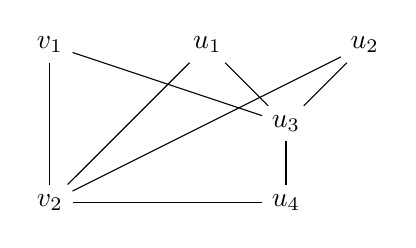
\begin{tikzpicture}
    \node (v1) at (0, 2) {\(v_1\)};
    \node (v2) at (0, 0) {\(v_2\)};
    \draw (v1) -- (v2);
    \node (u1) at (2, 2) {\(u_1\)};
    \node (u2) at (4, 2) {\(u_2\)};
    \node (u3) at (3, 1) {\(u_3\)};
    \node (u4) at (3, 0) {\(u_4\)};
    \draw (u1) -- (u3);
    \draw (u2) -- (u3);
    \draw (u4) -- (u3);
    \draw (v1) -- (u3);
    \draw (v2) -- (u1);
    \draw (v2) -- (u2);
    \draw (v2) -- (u4);
\end{tikzpicture}
\caption{\(\Theta_4\)}
\label{fig:Theta_4}
\end{figure}

\begin{thm}
    If \(\DConf_3(\Gamma)\) is a surface then \(\Gamma\) is either \(K_5\) or the \(\Theta_4\) graph.
\end{thm}
\begin{proof}
    Let \(v_1\) and \(v_2\) be adjacent vertices in \(\Gamma\).
    First, suppose \(\Gamma - \{v_1, v_2\}\) is a \(3\)-cycle, then \(\Gamma\) has \(5\) vertices.
    If \(\Gamma\) is not \(K_5\) then there are two vertices: \(v_i\), and \(u_1\) in \(\Gamma - \{v_1, v_2\}\)
    such that they are not connected by an edge in \(\Gamma\).
    Let \(u_2\) and \(u_3\) be the other two vertices in \(\Gamma - \{v_1, v_2\}\).
    Notice that \(\Gamma - \{u_2, u_3\}\) cannot be either a \(3\)-cycle nor a \(Y\)-graph.

    Suppose instead that \(\Gamma - v_1 v_2\) is a \(Y\)-graph, then \(\Gamma\) has \(6\) vertices.
    Since \(\Gamma\) is connected there exists at least one edge in \(\Gamma\) connecting \(v_1 v_2\) to \(\Gamma - v_1 v_2\).
    We then have one of the following in Figure \ref{fig:edgeygraphconnections}.
    \begin{figure}
        \centering
        \begin{tikzpicture}
            \node (v1) at (0, 2) {\(v_1\)};
            \node (v2) at (0, 0) {\(v_2\)};
            \draw (v1) -- (v2);
            \node (u1) at (2, 2) {\(u_1\)};
            \node (u2) at (4, 2) {\(u_2\)};
            \node (u3) at (3, 1) {\(u_3\)};
            \node (u4) at (3, 0) {\(u_4\)};
            \draw (u1) -- (u3);
            \draw (u2) -- (u3);
            \draw (u4) -- (u3);
            \draw (v1) -- (u1);
        \end{tikzpicture}
        \quad
        \begin{tikzpicture}
            \node (v1) at (0, 2) {\(v_1\)};
            \node (v2) at (0, 0) {\(v_2\)};
            \draw (v1) -- (v2);
            \node (u1) at (2, 2) {\(u_1\)};
            \node (u2) at (4, 2) {\(u_2\)};
            \node (u3) at (3, 1) {\(u_3\)};
            \node (u4) at (3, 0) {\(u_4\)};
            \draw (u1) -- (u3);
            \draw (u2) -- (u3);
            \draw (u4) -- (u3);
            \draw (v1) -- (u3);
        \end{tikzpicture}
        \caption{Possible ways to connect an edge to a \(Y\)-graph}
        \label{fig:edgeygraphconnections}
    \end{figure}

    Suppose that there is an edge in \(\Gamma\) between \(v_1\) and \(u_1\).
    Applying Lemma \ref{lem:is_surface_Y} to \(\Gamma - \{u_3, u_4\}\), we see there must be an edge
    connecting \(v_1\) and \(u_2\) in \(\Gamma\).
    Applying Lemma \ref{lem:is_surface_Y} to \(\Gamma - \{u_1, u_3\}\), there must be an edge between
    \(v_1\) and \(u_4\) in \(Gamma\).
    Finally, applying Lemma \ref{lem:is_surface_Y} to \(\Gamma - \{v_1, u_1\}\), there must must be
    an edge between \(v_2\) and \(u_2\).
    So in this case, \(\Gamma\) must have \(\Theta_4\) as a subgraph.

    Suppose instead that there is an edge in \(\Gamma\) between \(v_1\) and \(u_3\).
    Applying Lemma \ref{lem:is_surface_Y} to \(\Gamma - \{u_3, u_4\}\),
    we have two subcases.
    \begin{enumerate}
        \item There are edges \(v_1 u_1\) and \(v_1 u_2\) in \(\Gamma\).
        \item There are edges \(v_2 u_1\) and \(v_2 u_2\) in \(\Gamma\).
    \end{enumerate}
    In the second subcase if we apply Lemma \ref{lem:is_surface_Y} to \(\Gamma - \{u_1, u_3\}\),
    we see there must be an edge between \(v_1\) and \(u_4\) in \(\Gamma\).
    So, in this subcase, \(\Gamma\) must have \(\Theta_4\) as a subgraph.
    Suppose the first subcase is true, then applying Lemma \ref{lem:is_surface_Y} to \(\Gamma - \{u_2, u_3\}\),
    it follows that there is an edge between \(v_1\) and \(u_4\) in \(\Gamma\).
    Applying Lemma \ref{lem:is_surface_Y} to \(\Gamma - \{v_1, u_3\}\),
    we have two possibilities.
    \begin{enumerate}
        \item \(v_2\) is the center of the \(Y\)-graph \(\Gamma - \{v_1, u_3\}\).
        \item \(v_2\) is not the center of the \(Y\)-graph \(\Gamma - \{v_1, u_3\}\).
    \end{enumerate}
    If \(v_2\) is the center, then there must be edges \(v_2 u_1\), \(v_2, u_2\), \(v_2 u_4\) in \(\Gamma\).
    Putting particles at the vertices \(v_2\), \(u_2\), and \(u_4\), each of these particles can move
    simultaneously to \(u_1\), \(v_1\), and \(u_3\) respectively.
    This results in \((v_2, u_2, u_4)\) forming the corner of a \(3\)-cube in the configuration space
    contradicting that \(\DConf_3(\Gamma)\) is a surface.

    So, suppose that \(v_2\) is not the center of the \(Y\)-graph. Let \(u_i\) be the center of the \(Y\)-graph.
    Then, there must be an edge connecting \(v_2\) to \(u_i\).
    Putting particles at the vertices \(v_2\), \(u_j\), and \(u_k\) where \(j \neq i\) and \(k \neq i\),
    each of these particles can move simultaneously to \(u_i\), \(v_1\), and \(u_3\) respectively.
    Similarly this results in \((v_2, u_2, u_4)\) forming the corner of a \(3\)-cube in the configuration space.
    Therefore, \(\Gamma\) must have \(\Theta_4\) as a subgraph.

    It remains to show that \(\Gamma\) must equal \(\Theta_4\). Since \(\Gamma\) has \(\Theta_4\) as a subgraph
    if \(\Gamma\) is not \(\Theta_4\) this is equivalent to assuming there is at least one additional edge in \(\Theta_4\).
    So, if we just look at adding in one additional edge we have two possibilities (up to isomorphism).
    \begin{enumerate}
        \item There is an edge between \(v_2\) and \(u_3\).
        \item There is an edge between \(u_1\) and \(u_2\).
    \end{enumerate}
    In the second case, since \(\Gamma - \{u_1, u_2\}\) contains a \(4\)-cycle, Lemma \ref{lem:is_surface_Y} immediately fails.
    So suppose that there is an edge between \(v_2\) and \(u_4\).
    Applying Lemma \ref{lem:is_surface_Y} to \(\Gamma - \{v_2, u_4\}\), we see there must be additional edges to make \(\Gamma - \{v_2, u_3\}\)
    a \(Y\)-graph.
    There are two possibilities.
    \begin{enumerate}
        \item \(v_1\) is the center of the \(Y\)-graph \(\Gamma - \{v_2, u_3\}\).
        \item \(u_i\) is the center of the \(Y\)-graph \(\Gamma - \{v_2, u_3\}\) for some \(i \neq 3\).
    \end{enumerate}
    In either case there must be some edge connecting \(v_1\) to \(u_j\) for some \(j \neq 3\).
    Without a loss of generality suppose \(j = 1\).
    Then, immediately one can see that Lemma \ref{lem:is_surface_Y} fails for \(\Gamma - \{u_3, u_4\}\)
    as what remains contains a \(3\)-cycle.
    Therefore \(\Gamma\) must be \(\Theta_4\).
\end{proof}

\begin{thm}
    If \(\DConf_n(\Gamma)\) is a surface and \(n > 3\), then \(n = 4\) and \(\Gamma = K_{3,3}\).
\end{thm}
\begin{proof}
    Let \(v_1\) and \(v_2\) be adjacent vertices in \(\Gamma\).
    Since \(n > 3\), Lemma \ref{lem:is_surface_2} guarantees that \(\Gamma - \{v_1, v_2\}\) cannot be a \(Y\)-graph.
    So, \(\Gamma - \{v_1, v_2\}\) must be an \(n\)-cycle.
    Let \(u_1, u_2, \cdots, u_n\) be the vertices on the \(n\) cycle.
    Since \(\Gamma\) is connected there must be some edge connecting either \(v_1\) or \(v_2\) to some \(u_i\).
    Without a loss of generality suppose that \(v_1\) is connected to \(u_1\).
    If \(n > 4\) apply Lemma \ref{lem:is_surface_C} to \(\Gamma - \{v_1, u_1\}\) and see that
    \(u_2\) and \(u_n\) must connect to \(v_2\) in \(\Gamma\).
    Now put particles at each vertex in \(\{v_1, u_1, u_2, \cdots, u_n\}\setminus\{u_4\}\).
    As the particle at \(u_3\) moves to \(u_4\), any one of the particles at \(v_1\), \(u_2\), or \(u_n\) 
    can move to \(v_2\). These particles movements correspond to a book in the configuration space
    whose spine corresponds to the movement of the particle at \(u_3\) to \(u_4\).
    Therefore \(n\) must equal \(4\).
    See Figure \ref{fig:edge4cycle} for the current situation.
    Applying Lemma \ref{lem:is_surface_C} to \(\Gamma - \{v_1, u_1\}\), there must be an edges
    \(v_2 u_2\) and \(v_2 u_4\) in \(\Gamma\).
    Applying Lemma \ref{lem:is_surface_C} to \(\Gamma - \{v_2, u_2\}\), there must be an edge connecting \(v_1\)
    and \(u_2\).
    Therefore \(\Gamma\) must have \(K_{3,3}\) as a subgraph.

    Suppose that \(\Gamma\) was not \(K_{3,3}\).
    Then there is at least one additional edge.
    Without a loss of generality suppose this edge is \(u_2, u_4\).
    Then, \(\Gamma - \{v_1, u_3\}\) contains a \(3\)-cycle contradicting Lemma \ref{lem:is_surface_C}.
    Hence \(\Gamma\) must be \(K_{3,3}\).
    \begin{figure}[h!]
        \centering
        \begin{tikzpicture}
            \node (v1) at (0, 2) {\(v_1\)};
            \node (v2) at (0, 0) {\(v_2\)};
            \node (u1) at (3, 2) {\(u_1\)};
            \node (u2) at (2, 1) {\(u_2\)};
            \node (u4) at (4, 1) {\(u_4\)};
            \node (u3) at (3, 0) {\(u_3\)};
            \draw (v1) -- (v2);
            \draw (u1) -- (u2);
            \draw (u2) -- (u3);
            \draw (u3) -- (u4);
            \draw (u4) -- (u1);

            \draw (v1) -- (u1);
        \end{tikzpicture}
        \caption{Edge connected to \(4\)-cycle}
        \label{fig:edge4cycle}
    \end{figure}

    \begin{figure}
        \centering
        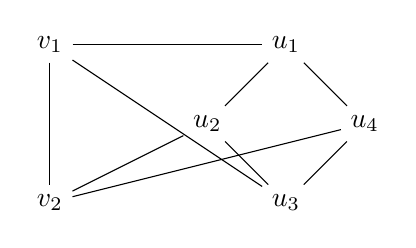
\begin{tikzpicture}
            \node (v1) at (0, 2) {\(v_1\)};
            \node (v2) at (0, 0) {\(v_2\)};
            \node (u1) at (3, 2) {\(u_1\)};
            \node (u2) at (2, 1) {\(u_2\)};
            \node (u4) at (4, 1) {\(u_4\)};
            \node (u3) at (3, 0) {\(u_3\)};
            \draw (v1) -- (v2);
            \draw (u1) -- (u2);
            \draw (u2) -- (u3);
            \draw (u3) -- (u4);
            \draw (u4) -- (u1);
            \draw (v1) -- (u1);
            \draw (v1) -- (u3);
            \draw (v2) -- (u2);
            \draw (v2) -- (u4);
        \end{tikzpicture}
        \label{fig:K3,3}
        \caption{\(K_{3,3}\)}
    \end{figure}

\end{proof}



% Used in 0-abstract.tex to get the length of the thesis.
\label{LastPage}

% Bibliography
{
    \singlespacing
    \bibliographystyle{abbrv}
    \bibliography{bibliography}
}
\end{document}